% Technical report of the C++ implementation of Stage 1.
% Build from cpp/docs/report/:
%   uv run --with matplotlib python charts.py     (figures/*.pdf, from cpp/benchmarks/results/)
%   tectonic report.tex                            (or pdflatex report.tex twice, for the contents)
% The finished report is copied to cpp/docs/Stage1_Cpp_Report.pdf.
\documentclass[11pt,a4paper]{article}

\usepackage[utf8]{inputenc}
\usepackage[T1]{fontenc}
\usepackage{lmodern}
\usepackage{microtype}
\usepackage[margin=2.4cm,headheight=14pt]{geometry}
\usepackage{graphicx}
\usepackage{booktabs}
\usepackage{tabularx}
\usepackage{array}
\usepackage{enumitem}
\usepackage{float}
\usepackage{xcolor}
\usepackage{listings}
\usepackage{tikz}
\usetikzlibrary{positioning,arrows.meta,calc}
\usepackage{fancyhdr}
\usepackage{titlesec}
\usepackage[hidelinks]{hyperref}

\definecolor{accent}{HTML}{2a78d6}
\definecolor{ink}{HTML}{0b0b0b}
\definecolor{muted}{HTML}{52514e}
\definecolor{codebg}{HTML}{f6f6f4}
\definecolor{rule}{HTML}{d8d7d2}
\definecolor{notebg}{HTML}{eef4fc}

\hypersetup{colorlinks=true,linkcolor=accent,urlcolor=accent,citecolor=accent}

\titleformat{\section}{\Large\bfseries\color{ink}}{\thesection.}{0.6em}{}
\titleformat{\subsection}{\large\bfseries\color{ink}}{\thesubsection}{0.6em}{}
\titleformat{\subsubsection}{\normalsize\bfseries\color{ink}}{\thesubsubsection}{0.6em}{}
\titlespacing*{\section}{0pt}{1.6em}{0.7em}
\titlespacing*{\subsection}{0pt}{1.2em}{0.5em}

\pagestyle{fancy}
\fancyhf{}
\fancyhead[L]{\small\color{muted}Stage 1 $\cdot$ Data layer $\cdot$ C++ implementation}
\fancyhead[R]{\small\color{muted}Big Data $\cdot$ ULPGC}
\fancyfoot[C]{\small\thepage}
\renewcommand{\headrulewidth}{0.4pt}

\setlist{itemsep=2pt,topsep=4pt}
\setlength{\parskip}{0.45em}
\setlength{\parindent}{0pt}
\setlength{\emergencystretch}{3em}
\renewcommand{\arraystretch}{1.25}

\lstdefinestyle{cpp}{
  language=C++, basicstyle=\ttfamily\footnotesize, backgroundcolor=\color{codebg},
  keywordstyle=\color{accent}\bfseries, commentstyle=\color{muted}\itshape,
  stringstyle=\color{ink}, frame=single, rulecolor=\color{rule}, framesep=4pt,
  xleftmargin=6pt, xrightmargin=6pt, breaklines=true, columns=fullflexible,
  keepspaces=true, showstringspaces=false, aboveskip=8pt, belowskip=8pt}
\lstdefinestyle{shell}{
  language={}, basicstyle=\ttfamily\footnotesize, backgroundcolor=\color{codebg}, frame=single,
  rulecolor=\color{rule}, framesep=4pt, xleftmargin=6pt, xrightmargin=6pt,
  breaklines=true, columns=fullflexible, keepspaces=true, showstringspaces=false,
  aboveskip=8pt, belowskip=8pt}
\lstset{style=cpp}

\newcolumntype{Y}{>{\raggedright\arraybackslash}X}
\newcolumntype{L}[1]{>{\raggedright\arraybackslash}p{#1}}
\newcommand{\code}[1]{\texttt{#1}}
\newcommand{\us}{\,$\mu$s}
\newenvironment{note}{\par\smallskip\noindent
\begin{tikzpicture}\node[fill=notebg,draw=accent!40,rounded corners=2pt,inner sep=7pt,text width=\dimexpr\linewidth-14pt\relax]\bgroup\small}{\egroup;\end{tikzpicture}\par\smallskip}

% One class card in the code walkthrough: \cls{Name}{kind}
\newcommand{\cls}[2]{\par\medskip\noindent{\large\bfseries\code{#1}}\hspace{0.6em}{\small\color{muted}#2}\par\nopagebreak\smallskip}
\newcommand{\why}[1]{\par\noindent\textit{Design rationale.} #1\par}

\begin{document}

% ---------------------------------------------------------------- title page
\hypersetup{pageanchor=false}
\begin{titlepage}
\thispagestyle{empty}
\vspace*{2.5cm}
{\color{accent}\rule{\linewidth}{1.2pt}}\\[0.8cm]
{\Huge\bfseries Search Engine Project\par}
\vspace{0.4cm}
{\LARGE Stage 1: Building the Data Layer\par}
\vspace{0.6cm}
{\Large\color{muted} C++ implementation --- technical report\par}
\vspace{0.6cm}
{\color{accent}\rule{\linewidth}{1.2pt}}
\vspace{2cm}

\begin{tabular}{@{}>{\bfseries}L{3.4cm}L{10.5cm}@{}}
Course & Big Data $\cdot$ Grado en Ciencia e Ingeniería de Datos $\cdot$ Universidad de Las Palmas de Gran Canaria \\
Academic year & 2026/2027 \\
Group name & BigData-Ulpgc \\
Members & Carlos Falcón Brito --- C++ implementation, author of this report \\
 & Daniel Rodríguez Alonso --- Java implementation \\
 & Daniel Perdomo Medina --- Python implementation \\
Repository & \url{https://github.com/BigData-Ulpgc/stage_1}, folder \code{cpp/} \\
Status & Complete pipeline, offline mode with the sample dataset, structures chosen by configuration, 12 benchmark experiments, 232 tests passing \\
Date & 4 October 2026 \\
\end{tabular}

\vfill
\begin{note}
\textbf{Quick check for instructors.} From \code{cpp/}, with a C++20 compiler, CMake, Ninja, SQLite3,
libcurl and mongo-cxx-driver installed, and no network: \code{make}, then
\code{./build/release/search\_engine\_stage1 pipeline 30 -{}-offline} and
\code{./build/release/search\_engine\_stage1 search whale island}. Section~\ref{sec:quick} gives the
exact commands and the expected output.
\end{note}
\end{titlepage}
\hypersetup{pageanchor=true}

% ---------------------------------------------------------------- abstract + toc
\section*{Abstract}
This report describes the C++ implementation of Stage~1 of the group's search engine over Project
Gutenberg books. Stage~1 builds the \emph{data layer}: a pipeline that downloads books, splits each
one into header and body, stores them in a datalake, extracts their metadata into a SQLite datamart
and builds an inverted index that answers Boolean AND queries. A control layer records the progress,
so an interrupted run resumes without losing or repeating books.

The module offers three datalake layouts (\code{book}, \code{range}, \code{time}) and three persistent
inverted-index structures (\code{monolithic} JSON, \code{hierarchical} folders, \code{mongo}),
selectable through a configuration file without recompiling. It follows the group's common
contract (\code{shared/SPEC.md}): it reproduces the reference term counts of the shared dataset
exactly and stores byte-identical books. A 15-book sample dataset lets the whole pipeline run
offline in under half a second. The 12 benchmark experiments, run on the 200 real books of the dataset,
lead to \code{book} + \code{monolithic} for the final system. They also show that the
\code{monolithic} index is the fastest to build and to query, but its update cost and memory grow with
the index; that \code{hierarchical} reserves 73 times its data size in file-system blocks; and that
SQLite's \code{author} and \code{title} indexes keep metadata lookups flat as the table grows.

\tableofcontents
\newpage

% ================================================================ 1
\section{Introduction and objectives}

\subsection{Goal of Stage 1}
The project builds a search engine over books from Project Gutenberg in several stages. Stage~1
builds the data layer that the later stages query. Table~\ref{tab:layers} lists its parts.

\begin{table}[H]
\centering\small
\begin{tabularx}{\linewidth}{@{}L{3.4cm} Y@{}}
\toprule
Part & What it does \\
\midrule
Crawler & Downloads a book and splits it into header and body at the START/END markers, dropping the license footer. \\
Datalake & Stores the raw books in one of three folder layouts. \\
Metadata datamart & Keeps title, author, language and release date of every book in SQLite. \\
Inverted-index datamart & Maps each term to the sorted ids of the books that contain it, in one of three structures. \\
Query & Answers a query with the books that contain \emph{every} term (AND semantics). \\
Control layer & Records which books are downloaded and which are indexed, so a run can resume. \\
\bottomrule
\end{tabularx}
\caption{The parts of the Stage~1 data layer.}
\label{tab:layers}
\end{table}

\subsection{The group and the common contract}
The same data layer is implemented three times, in Java, Python and C++, one implementation per
member. All three follow \code{shared/SPEC.md}, so they process the same dataset with the same rules
and produce equivalent outputs. Table~\ref{tab:spec} lists what the contract fixes.

\begin{table}[H]
\centering\small
\begin{tabularx}{\linewidth}{@{}L{1.2cm} L{3.6cm} Y@{}}
\toprule
SPEC & Topic & What it fixes \\
\midrule
\S1 & Dataset & 200 Gutenberg ids in \code{shared/book\_ids.txt}; the query workload; the stopwords. \\
\S2 & Download and split & The URL, the START/END markers, header and body trimmed, \code{\textbackslash r\textbackslash n} normalised to \code{\textbackslash n}. \\
\S3 & Datalake layouts & \code{book}: \code{<ID>/body.txt}; \code{range}: \code{01000-01999/<ID>.body.txt}; \code{time}: \code{YYYYMMDD/HH/<ID>.body.txt}. \\
\S4 & Metadata & Four regular expressions and the SQLite table \code{books}, with indexes on \code{author} and \code{title}. \\
\S5 & Tokenizer & ASCII letters and digits only, lower case, tokens of two or more characters, stopwords removed. \\
\S6 & Index structures & The monolithic JSON file, the hierarchical folders and the MongoDB collection. \\
\S7 & Queries & AND semantics; result in ascending id order. \\
\S8 & Control layer & An id is written only after its step succeeded. \\
\S9--10 & Benchmarks & The CSV format, 2 warm-ups and 5 measured runs, and the data and sizes of each experiment. \\
\bottomrule
\end{tabularx}
\caption{What the common contract fixes for every implementation.}
\label{tab:spec}
\end{table}

\subsection{Objectives and scope of this report}
\begin{itemize}
  \item Describe the architecture of the C++ module and how a book moves through it.
  \item Justify the design decisions, including the structures selected for the final implementation.
  \item Walk through the modules and their classes.
  \item Explain how the module is tested, built and run.
  \item Present and discuss the results of the 12 benchmark experiments.
\end{itemize}
C++ was chosen for this implementation because the data layer is dominated by text processing, file
input/output and in-memory data structures: C++ gives direct control over memory and over every
system call, and makes those costs visible in the benchmarks. The full record of how the module was
built, step by step and with the reason behind every choice, is in \code{cpp/docs/DEVLOG.md}; the
build and usage details are in \code{cpp/docs/USER\_GUIDE.md}.

% ================================================================ 2
\section{System architecture}

Figure~\ref{fig:components} follows one book through the module. Every storage box is an
interface with several interchangeable implementations.

\begin{figure}[H]
\centering
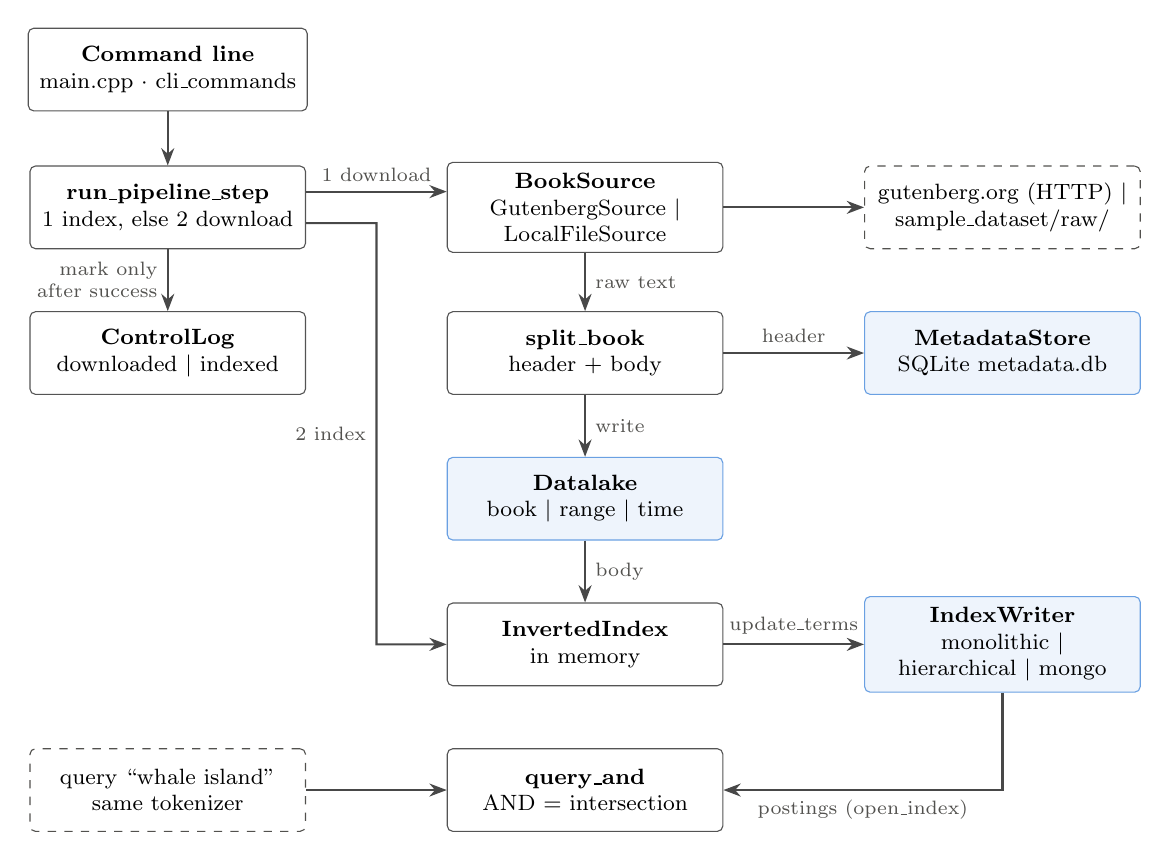
\begin{tikzpicture}[
  font=\footnotesize,
  box/.style={draw=ink!70,rounded corners=2pt,align=center,minimum height=1.05cm,inner sep=4pt,fill=white,minimum width=3.5cm},
  store/.style={box,fill=notebg,draw=accent!70},
  ext/.style={box,dashed,draw=muted},
  arr/.style={-{Stealth[length=2.2mm]},thick,draw=ink!75},
  lbl/.style={font=\scriptsize,color=muted}]
  \node[box] (cli) at (0,1.75) {\textbf{Command line}\\main.cpp $\cdot$ cli\_commands};
  \node[box] (step) at (0,0) {\textbf{run\_pipeline\_step}\\1 index, else 2 download};
  \node[box] (ctrl) at (0,-1.85) {\textbf{ControlLog}\\downloaded $|$ indexed};
  \node[ext] (q) at (0,-7.4) {query ``whale island''\\same tokenizer};
  \node[box] (src) at (5.3,0) {\textbf{BookSource}\\GutenbergSource $|$\\LocalFileSource};
  \node[box] (split) at (5.3,-1.85) {\textbf{split\_book}\\header + body};
  \node[store] (lake) at (5.3,-3.7) {\textbf{Datalake}\\book $|$ range $|$ time};
  \node[box] (inv) at (5.3,-5.55) {\textbf{InvertedIndex}\\in memory};
  \node[box] (qa) at (5.3,-7.4) {\textbf{query\_and}\\AND = intersection};
  \node[ext] (net) at (10.6,0) {gutenberg.org (HTTP) $|$\\sample\_dataset/raw/};
  \node[store] (meta) at (10.6,-1.85) {\textbf{MetadataStore}\\SQLite metadata.db};
  \node[store] (wr) at (10.6,-5.55) {\textbf{IndexWriter}\\monolithic $|$\\hierarchical $|$ mongo};

  \draw[arr] (cli) -- (step);
  \draw[arr] ([yshift=2mm]step.east) -- node[above,lbl]{1 download} ([yshift=2mm]src.west);
  \draw[arr] (src) -- (net);
  \draw[arr] (src) -- node[right,lbl]{raw text} (split);
  \draw[arr] (split) -- node[right,lbl]{write} (lake);
  \draw[arr] (split) -- node[above,lbl]{header} (meta);
  \draw[arr] (step) -- node[left,lbl,align=right]{mark only\\after success} (ctrl);
  \draw[arr] ([yshift=-2mm]step.east) -- (2.65,-0.2) -- node[pos=0.5,left,lbl]{2 index} (2.65,-5.55) -- (inv.west);
  \draw[arr] (lake) -- node[right,lbl]{body} (inv);
  \draw[arr] (inv) -- node[above,lbl]{update\_terms} (wr);
  \draw[arr] (wr.south) |- node[pos=0.75,below,lbl]{postings (open\_index)} (qa.east);
  \draw[arr] (q) -- (qa);
\end{tikzpicture}
\caption{Main components and data flow. \code{cli\_commands} builds every piece from the
configuration, using \code{create\_datalake} and \code{create\_index\_writer}.}
\label{fig:components}
\end{figure}

\subsection{The life of a book}
\begin{enumerate}
  \item \code{run\_pipeline\_step} asks \code{next\_control\_action}, which reads only the two control
        logs. No book is waiting to be indexed, so it picks the first id of \code{book\_ids.txt}
        that is not downloaded yet, for example 1342.
  \item \code{BookSource::fetch(1342)} returns a \code{DownloadResult}: \code{GutenbergSource}
        downloads the \code{.txt} over HTTP with libcurl, or \code{LocalFileSource} reads it from the
        sample dataset. \code{split\_book} finds the markers and returns a \code{SplitBook} with the
        header and the body; a book without both markers is discarded.
  \item \code{Datalake::write} stores header and body and returns a \code{BookLocation}.
        \code{extract\_metadata} parses the header, and \code{MetadataStore::insert\_book} saves the
        row together with the two paths.
  \item Only if all of this succeeded does \code{ControlLog::mark} record 1342 in the download log,
        \code{downloaded\_books.txt}.
  \item The next step finds a downloaded book that is not indexed. It reads the body through the path
        stored in SQLite, tokenizes it, adds the book's distinct terms to the in-memory
        \code{InvertedIndex}, and persists only those terms with \code{IndexWriter::update\_terms}.
  \item Only then is 1342 appended to \code{indexed\_books.txt}.
  \item A query ``whale island'' is tokenized like a book; \code{query\_and} asks the configured index
        for the posting lists of \code{whale} and \code{island} and intersects them, starting with the
        shortest.
\end{enumerate}

\subsection{Layers and dependencies}
Dependencies always point downwards: a module only uses the modules below it
(Figure~\ref{fig:layers}). The orchestration code depends on interfaces (\code{Datalake},
\code{IndexWriter}, \code{BookSource}, \code{HttpClient}, \code{Clock}); only the command line and the
factories know which concrete class is used.

\begin{figure}[H]
\centering
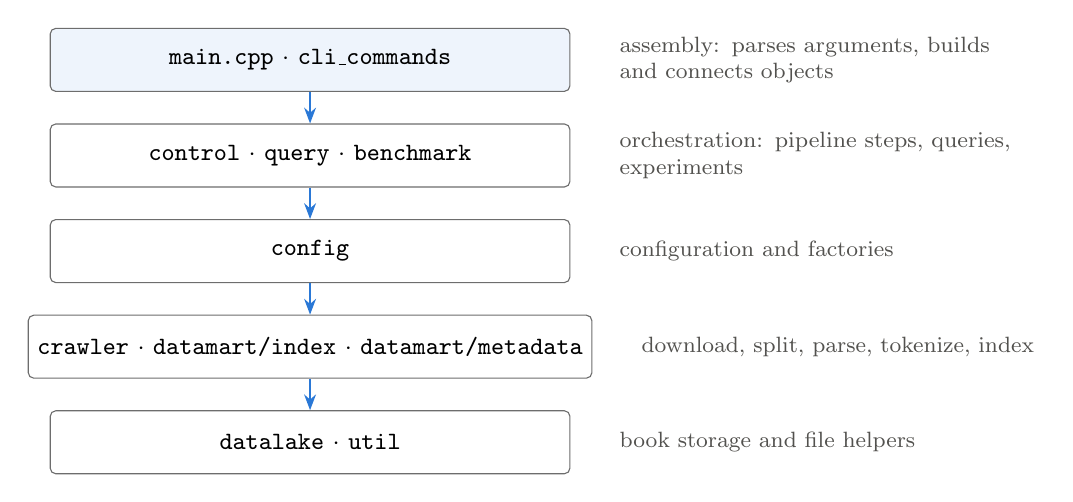
\begin{tikzpicture}[font=\small,
  layer/.style={draw=ink!60,rounded corners=2pt,minimum width=6.6cm,minimum height=0.8cm,fill=white},
  arr/.style={-{Stealth[length=2mm]},thick,draw=accent}]
  \node[layer,fill=notebg] (a) {\code{main.cpp} $\cdot$ \code{cli\_commands}};
  \node[layer,below=0.4cm of a] (b) {\code{control} $\cdot$ \code{query} $\cdot$ \code{benchmark}};
  \node[layer,below=0.4cm of b] (c) {\code{config}};
  \node[layer,below=0.4cm of c] (d) {\code{crawler} $\cdot$ \code{datamart/index} $\cdot$ \code{datamart/metadata}};
  \node[layer,below=0.4cm of d] (e) {\code{datalake} $\cdot$ \code{util}};
  \foreach \x/\y in {a/b,b/c,c/d,d/e} \draw[arr] (\x) -- (\y);
  \node[right=0.5cm of a,text width=5.0cm,color=muted,font=\footnotesize] {assembly: parses arguments, builds and connects objects};
  \node[right=0.5cm of b,text width=5.0cm,color=muted,font=\footnotesize] {orchestration: pipeline steps, queries, experiments};
  \node[right=0.5cm of c,text width=5.0cm,color=muted,font=\footnotesize] {configuration and factories};
  \node[right=0.5cm of d,text width=5.0cm,color=muted,font=\footnotesize] {download, split, parse, tokenize, index};
  \node[right=0.5cm of e,text width=5.0cm,color=muted,font=\footnotesize] {book storage and file helpers};
\end{tikzpicture}
\caption{Module layers. Each one only uses the layers below it.}
\label{fig:layers}
\end{figure}

\subsection{Design principles applied throughout}
\begin{table}[H]
\centering\small
\begin{tabularx}{\linewidth}{@{}L{3.1cm} Y Y@{}}
\toprule
Principle & Where & Why \\
\midrule
Programming to interfaces & \code{Datalake}, \code{IndexWriter}, \code{BookSource}, \code{HttpClient}, \code{Clock} & Changing a structure does not touch its users; the tests plug in fakes. \\
Dependency injection & \code{run\_pipeline\_step} receives every collaborator by reference; \code{TimeBasedDatalake} receives its \code{Clock}. & Nothing is created behind the scenes; any piece can be replaced in tests and benchmarks. \\
Factories & \code{create\_datalake}, \code{create\_index\_writer}, \code{open\_index} & One configuration name $\rightarrow$ one class, in a single place. \\
RAII & \code{MetadataStore} (\code{sqlite3*}), \code{Statement}, \code{CurlHandle}, the tests' \code{TempDir} & Resources are released on every path out of a function, exceptions included. \\
Pure decisions & \code{next\_control\_action}, \code{split\_book}, \code{extract\_metadata}, \code{tokenize}, \code{query\_and} & The logic that decides is tested without disk or network. \\
Mark after doing & \code{run\_pipeline\_step}: \code{ControlLog::mark} only after the step succeeded. & The control layer never claims what did not happen; at worst a step is repeated. \\
Value types & \code{SplitBook}, \code{BookLocation}, \code{StoredBook}, \code{StepResult}, \code{AppConfig} & Plain data without behaviour, copied or moved, never shared by accident. \\
Fail fast, absence explicit & Configuration checked at start-up; \code{std::optional} for a missing marker or book; exceptions for I/O errors. & A wrong configuration stops the program before it writes anything; expected absence is never an error code. \\
\bottomrule
\end{tabularx}
\caption{Design principles and where they appear in the code.}
\end{table}

\subsection{Project organisation}

\subsubsection{Folder tree}
The three source trees share one layout, one folder per module, so a header, its source and its
tests are always found at the same relative path.
\begin{lstlisting}[style=shell]
cpp/
  CMakeLists.txt, CMakePresets.json, Makefile   build: library, executable, tests
  config.properties                             the structures pipeline and search use
  include/stage1/   util/ crawler/ datalake/ datamart/{metadata,index}/ query/
                    control/ config/ benchmark/{datalake,index,metadata}/ cli_commands.hpp
  src/              the same folders; main.cpp, cli_commands.cpp
  tests/            the same folders; fakes/ (FakeHttpClient, FakeClock), support/ (TempDir)
  benchmarks/results/   real/{datalake,index}/ and synthetic/metadata/ CSVs (committed)
  docs/             USER_GUIDE.md, DEVLOG.md, this report and its sources (report/)
  data/             written by the pipeline (git-ignored)
\end{lstlisting}

\subsubsection{Build targets and dependencies}
\begin{table}[H]
\centering\small
\begin{tabularx}{\linewidth}{@{}L{4.0cm} Y@{}}
\toprule
Target & Contents \\
\midrule
\code{stage1\_core} & Static library with all the logic: every module except the command line. \\
\code{search\_engine\_stage1} & The executable: \code{main.cpp} and \code{cli\_commands.cpp}. It alone receives the build-time paths of \code{shared/}, \code{data/}, \code{benchmarks/} and \code{config.properties}, so it runs from any folder. \\
\code{stage1\_tests} & One GoogleTest executable with the 232 tests, registered in CTest. \\
\bottomrule
\end{tabularx}
\caption{CMake targets. The presets \code{release} (benchmarks) and \code{debug} (development) configure Ninja builds; \code{make} and \code{make test} are shortcuts.}
\end{table}

\begin{table}[H]
\centering\small
\begin{tabularx}{\linewidth}{@{}L{3.4cm} L{4.0cm} Y@{}}
\toprule
Library & Obtained from & Used for \\
\midrule
SQLite3 & System (macOS SDK, \code{libsqlite3-dev}) & The metadata datamart. \\
libcurl & System & Downloading books over HTTP. \\
mongo-cxx-driver 4.x & Homebrew or the driver's sources & The \code{mongo} index structure. \\
nlohmann/json & CMake \code{FetchContent} & The monolithic JSON index. \\
GoogleTest & CMake \code{FetchContent} & The test suite. \\
\bottomrule
\end{tabularx}
\caption{External libraries.}
\end{table}

% ================================================================ 3
\section{Design decisions}\label{sec:decisions}

\subsection{Structures selected for the final implementation}
The final system uses \code{book} for the datalake and \code{monolithic} for the inverted index,
selected in \code{cpp/config.properties}. The benchmarks of Section~\ref{sec:bench} support both
choices at the project's 200 books.

\textbf{Datalake: \code{book}.}
\begin{itemize}
  \item \textbf{Lookup.} The fastest one that survives a restart: 2.52\us{} per book, against 2.92\us{}
        for \code{range}. A \code{book} path is computed from the id alone. \code{time} cannot compute
        a book's folder from its id; this module's 0.07\us{} comes from an in-memory map that a new
        process does not have, and a lookup that survives a restart has to scan the day and hour
        folders.
  \item \textbf{Detection and recovery.} The fastest detection of new books (0.98\,ms, against 1.16
        for \code{time} and 1.66 for \code{range}) and the fastest recovery after a crash (19.1\,ms,
        against 20.0 and 22.3).
  \item \textbf{Its one loss.} Writing all 200 books takes 228\,ms, against 192 for \code{range} and
        187 for \code{time}. The three layouts store identical bytes; \code{book} reserves 0.6\% more
        disk.
  \item \textbf{When it would change.} \code{book} adds one folder per book to the datalake's root
        (200 today). For a collection the size of the whole Gutenberg catalogue, \code{range} keeps
        the direct lookup and caps each folder at 1,000 books.
\end{itemize}

\textbf{Inverted index: \code{monolithic}.}
\begin{itemize}
  \item \textbf{Queries.} The fastest: 1.4\us{} per query, against 22.0\us{} for \code{hierarchical}
        and 314.6\us{} for \code{mongo}.
  \item \textbf{Build and update.} The fastest to build (1.8\,s, against 6.5 and 3.4\,s) and the
        cheapest to update at this size (300\,ms per added book, against 482 and 922\,ms).
  \item \textbf{Its costs grow with the index.} Adding a book costs 93, 165 and 300\,ms at
        $N = 50$, 100 and 200 (the whole file is rewritten), and keeping the index open takes 16.3,
        28.1 and 54.1\,MB. Extrapolating these three sizes in a straight line, \code{hierarchical}
        becomes the cheaper index to update at roughly 700 books. Past that point it is the natural
        next structure: it also beats \code{mongo} on both queries and updates.
\end{itemize}

\subsection{Implementation decisions}
\begin{table}[H]
\centering\small
\begin{tabularx}{\linewidth}{@{}L{3.9cm} L{3.2cm} Y@{}}
\toprule
Decision & Alternative discarded & Reason \\
\midrule
Each indexed book persists only its own terms (\code{update\_terms}) & Rewriting the whole index per book & The rewrite made \code{hierarchical} over 100 times slower than \code{monolithic}; updating only the changed terms was measured 3--4 times faster. \\
SQLite rows inserted in batches: one transaction and one prepared statement per batch, all or nothing & One commit per row & Committing every row was slow and noisy; batching was about 2.5 times faster, and a failed batch leaves nothing behind. \\
MongoDB updates sent as one unordered bulk write & One \code{update\_one} per term (about 7,900 round trips per book) & An index update went from 3,421\,ms to about 300\,ms per book. \\
Index rebuilt in memory at start-up, then compared with the stored structure & Trusting that the stored structure exists & A missing, partial or stale structure is rewritten whole. Found by testing: 5 stale documents in a Mongo collection made \code{search} answer from them. \\
The \code{time} layout's \code{locate} remembers the paths it wrote & Scanning the day and hour folders & Constant-time lookups. Indexing reads the body path from SQLite, so the pipeline never needs \code{locate} across runs. \\
Structures chosen in \code{config.properties}, overridable with \code{-Dkey=value} & Hardcoded structures; a flag on every command & One file keeps \code{pipeline} and \code{search} on the same index; a typo stops the program at start-up. \\
Paths fixed at build time & Paths relative to the working directory & The executable finds its files from any folder. \\
Offline source over \code{sample\_dataset/raw/} & Network-only pipeline & The whole pipeline runs in under half a second without network, and its output is compared byte for byte with the expected split. \\
Reproducible benchmarks: a simulated clock, a fixed-seed random generator, untimed preparation, verification before reporting & Real clock and ad-hoc randomness & Every repetition builds the same data, and every implementation makes the same ``random'' choices. \\
\bottomrule
\end{tabularx}
\caption{Implementation decisions. \code{cpp/docs/DEVLOG.md} records each one with its measurements.}
\end{table}

% ================================================================ 4
\section{Implementation: modules and classes}
This section walks through the modules from the bottom layer up. All code lives in the namespace
\code{stage1}.

\subsection{Module \code{util}: file and text helpers}
\cls{write\_text\_file / read\_text\_file}{free functions}
Write a string to a file, creating any missing parent folder first, and read a whole file back. Both
throw \code{std::runtime\_error} with the path when the file system fails.
\cls{collect\_body\_header\_pairs, count\_files\_with\_suffix, trim}{free functions}
Shared by the datalake layouts and the benchmarks: list the ids that have both a body and a header in
a folder, count files by suffix, and trim whitespace.
\why{Every layout writes files the same way; keeping that in one place means a single, tested
definition of ``write a file''.}

\subsection{Module \code{crawler}: fetching and splitting}
\cls{HttpClient}{interface}
One method, \code{get(url)}, returning a \code{DownloadResult}. \code{CurlHttpClient} implements it with
libcurl (following redirects, with an RAII \code{CurlHandle}); the tests use \code{FakeHttpClient}.
\cls{DownloadResult}{value type}
Either \code{success(text)} or \code{failure(message)}: a failed download is an expected outcome, not an
exception.
\cls{BookSource}{interface}
\code{fetch(book\_id)}. \code{GutenbergSource} builds the SPEC URL and calls an \code{HttpClient};
\code{LocalFileSource} reads \code{pg<ID>.txt} from a folder, which is the offline mode.
\cls{split\_book}{free function}
Normalises \code{\textbackslash r\textbackslash n} to \code{\textbackslash n}, finds the START and END
markers (``THE'' or ``THIS'' variant), and returns a \code{SplitBook} with the trimmed header and body,
or \code{std::nullopt} when a marker is missing.
\why{Where a book comes from is the only difference between the online and offline modes: both are
\code{BookSource}s, and nothing after \code{fetch} knows which one it was given.}

\subsection{Module \code{datalake}: storing the books}
\cls{Datalake}{interface}
Three operations: \code{write(id, header, body)} returns a \code{BookLocation} with both paths;
\code{locate(id)} finds a book; \code{list\_book\_ids()} walks the folders and returns every id with
both files.
\cls{BookBasedDatalake}{layout}
\code{<root>/<ID>/body.txt} and \code{header.txt}. The path is a pure function of the id.
\cls{RangeBasedDatalake}{layout}
\code{<root>/<INI>-<FIN>/<ID>.body.txt}, with \code{range\_folder\_name} computing the five-digit range
from the id.
\cls{TimeBasedDatalake}{layout}
\code{<root>/YYYYMMDD/HH/<ID>.body.txt}, the folder taken from an injected \code{Clock}:
\code{SystemClock} in production, \code{FakeClock} in the tests and a simulated clock in the
benchmarks. Since the path depends on \emph{when} the book was written, \code{locate} uses a map of the
paths this instance wrote.
\why{The interface is what the benchmarks plug the three layouts into; \code{list\_book\_ids} reads only
the disk, so it works from a new process and is what recovery and change detection rely on.}

\subsection{Module \code{datamart/metadata}: metadata in SQLite}
\cls{extract\_metadata}{free function}
Applies the four SPEC regular expressions (\code{std::regex}, multiline) to a header: first match,
first line of the value, trimmed. A missing field becomes \code{std::nullopt} and is stored as SQL
\code{NULL}.
\cls{MetadataStore}{class, owns a \code{sqlite3*}}
Creates the \code{books} table and its two indexes on first open. \code{insert\_book} inserts or
replaces one row; \code{insert\_books} inserts a batch in one transaction with one prepared statement,
rolling the whole batch back if a row fails; \code{count}, \code{find\_by\_id}, \code{find\_by\_author}
and \code{find\_by\_title} (exact match, ascending ids) read it back as \code{StoredBook} values.
\why{An RAII \code{Statement} wrapper finalises every prepared statement on every path; the
transaction methods are private, so a caller cannot leave a transaction open.}

\subsection{Module \code{datamart/index}: the inverted index}
\cls{tokenize, load\_stopwords}{free functions}
The SPEC tokenizer, byte by byte: \code{A--Z} lower-cased, \code{a--z} and \code{0--9} kept, any other
byte a separator, tokens shorter than two dropped, stopwords removed.
\cls{InvertedIndex}{class}
An \code{std::unordered\_map} from term to \code{std::set<int>}: \code{add\_book}, \code{postings}
(sorted, no duplicates), \code{term\_count} and \code{entries} (every term with its postings, in term
order).
\cls{IndexWriter}{interface}
\code{write(index)} makes a structure match the whole index; \code{update\_terms(index, terms)} persists
only the given terms. The default \code{update\_terms} calls \code{write}, which is all a single file can do.
\cls{MonolithicIndexWriter}{structure}
One JSON object \code{\{"term": [ids]\}} with nlohmann/json: keys sorted, compact output.
\cls{HierarchicalIndexWriter}{structure}
\code{inverted\_index/<FIRST LETTER>/<term>.txt}, one id per line. \code{write} replaces the folder;
\code{update\_terms} rewrites only the files of the given terms.
\cls{MongoIndexWriter}{structure}
One document \code{\{term, postings\}} per term with a unique index on \code{term}. \code{write} replaces
the collection with \code{insert\_many}; \code{update\_terms} sends one unordered bulk write of upserts.
The real index, the benchmarks and the tests use separate databases.
\cls{Readers}{free functions}
\code{monolithic\_postings\_fetcher} parses the JSON once; \code{hierarchical\_postings\_fetcher} reads
one file per lookup; \code{mongo\_postings\_fetcher} runs one query per term. Each returns the function
\code{query\_and} takes.
\why{Readers return a plain \code{std::function}, so querying an on-disk structure and querying the
in-memory index are the same code.}

\subsection{Module \code{query}: the search}
\cls{query\_and}{free function}
Takes the query's terms and a postings source, sorts the posting lists by length, and intersects them
starting from the shortest, stopping as soon as the result is empty. The result is sorted ascending.

\subsection{Module \code{control}: progress and recovery}
\cls{ControlLog}{class}
An append-only file of ids: \code{contains}, \code{mark} and \code{ids} (sorted).
\cls{next\_control\_action}{free function}
Pure: from the candidate ids and the two logs, decides \code{IndexBook} (the first downloaded book not
indexed), else \code{DownloadBook} (the first not downloaded), else \code{Nothing}.
\cls{run\_pipeline\_step}{free function}
Performs that decision against the components it receives and returns a \code{StepResult}: the decision,
whether it completed, and why not.
\why{Indexing goes first, so downloaded books never pile up unindexed; and marking only after success
is what makes an interrupted run safe to resume.}

\subsection{Module \code{config}: configuration and factories}
\cls{AppConfig, load\_config}{value type and function}
\code{datalake.structure} and \code{index.structure}: defaults, then \code{config.properties} if it
exists, then \code{-Dkey=value} overrides. An unknown key or value throws \code{std::invalid\_argument}.
\cls{create\_datalake}{factory}
The only place that turns a layout name into a class. A \code{time} datalake owns the clock it is
given through a private base class constructed before it, so the factory returns a plain
\code{std::unique\_ptr<Datalake>}.
\cls{create\_index\_writer, open\_index, index\_exists, stored\_term\_count}{factories}
The write and read sides of each index structure at its SPEC location, and the checks the pipeline
uses at start-up.

\subsection{Module \code{benchmark}}
\cls{measure\_elapsed\_ms, BenchmarkResult}{shared}
Runs an untimed setup and a timed operation, 2 warm-ups and 5 measured runs with a steady clock; the
rows are written in the SPEC CSV format.
\cls{JavaRandom, SimulatedClock}{reproducibility}
\code{JavaRandom} is a fully specified 48-bit linear congruential generator, the published algorithm
of \code{java.util.Random}, seeded with 42 and checked against reference values. The output of
the standard \code{<random>} distributions depends on the standard library, so they would give a
different lookup order and query workload with libc++ and with libstdc++; this generator gives the same
sequence on every platform. \code{SimulatedClock} advances six minutes per call, so the \code{time}
layout gets ten books per hour folder in every repetition.
\cls{datalake/, index/, metadata/}{experiments}
One file per experiment plus a support module each: \code{fresh\_datalake}, \code{tokenize\_all},
\code{build\_index} and \code{verify\_index}, \code{synthetic\_metadata} and
\code{fresh\_metadata\_store}.
\why{Every experiment verifies before it reports: a written index must answer like the in-memory one,
every lookup must find its book, a recovery must leave nothing lost or duplicated.}

\subsection{The command line}
\cls{main.cpp}{entry point}
Parses \code{-Dkey=value} overrides and the command, loads the configuration and dispatches.
\cls{cli\_commands}{commands}
\code{pipeline}, \code{search}, \code{status}, \code{config} and \code{benchmark}: each builds the real
components (paths fixed at build time) and drives the modules above.

% ================================================================ 5
\section{Testing strategy}
The suite has 232 GoogleTest tests (Table~\ref{tab:tests}), run with \code{make test}. No test uses the
network or the real \code{data/} folder: they use \code{FakeHttpClient}, \code{FakeClock} and temporary
folders that are deleted when the test ends.

\begin{table}[H]
\centering\small
\begin{tabularx}{\linewidth}{@{}L{3.6cm} r Y@{}}
\toprule
Area & Tests & What they check \\
\midrule
\code{benchmark/} & 71 & Rows, units and order of every experiment; \code{JavaRandom} against reference values; the simulated clock; each experiment's verification \\
\code{datamart/index/} & 49 & Tokenizer and stopwords; the in-memory index; every writer and reader, Mongo included \\
\code{datalake/} & 25 & Paths, \code{locate} and \code{list\_book\_ids} of the three layouts \\
\code{control/} & 24 & The control decision, the logs, and complete pipeline steps, failures included \\
\code{datamart/metadata/} & 22 & The four regular expressions; inserts, batches (all or nothing) and lookups \\
\code{crawler/} & 19 & Marker split, the download client, the offline source \\
\code{config/} & 12 & Configuration precedence and errors; both factories \\
\code{query/} & 7 & AND intersection and its edge cases \\
Smoke & 3 & The build links and runs \\
\bottomrule
\end{tabularx}
\caption{The test suite by area.}
\label{tab:tests}
\end{table}

\subsection{MongoDB tests}
The 11 tests that need MongoDB use their own database, \code{search\_engine\_test}, and are skipped
when no server answers, so the suite passes on a machine without Docker. Against the group's
container (MongoDB 8.2.12) all of them pass.

\subsection{The sample dataset test}
\code{LocalFileSource} is tested on the real \code{sample\_dataset/raw/} files: splitting each of the
15 books must reproduce \code{sample\_dataset/book/<ID>/} byte for byte. A full offline run checks the
same at the level of the whole datalake (Section~\ref{sec:quick}).

\subsection{Checks beyond the unit tests}
\begin{itemize}
  \item The index built from the $N$ books with the lowest ids has exactly the SPEC reference counts:
        58,834 / 78,820 / 129,356 terms and 360,970 / 759,087 / 1,581,064 postings for
        $N = 50$ / 100 / 200, the same counts the other two implementations produce.
  \item The datalake stores the same 128,980,349 bytes as the other implementations.
  \item A test that failed only on Linux, because it compared two allocations of a few hundred bytes,
        was reproduced in an Ubuntu 24.04 (glibc 2.39) container and fixed.
\end{itemize}

% ================================================================ 6
\section{Setup and execution}

\subsection{Requirements}
\begin{itemize}
  \item macOS: \code{xcode-select -{}-install}, then \code{brew install cmake ninja mongo-cxx-driver}.
  \item Linux (Ubuntu or Debian): the distribution's packages \code{build-essential}, \code{cmake},
        \code{ninja-build}, \code{libsqlite3-dev} and \code{libcurl4-openssl-dev}, plus
        mongo-cxx-driver 4.x.
  \item CMake downloads nlohmann/json and GoogleTest on the first build.
  \item MongoDB is optional; without a server its tests and benchmark rows are skipped.
\end{itemize}

\subsection{Build and test}
From the \code{cpp/} folder, \code{make} configures and builds the \code{release} preset with Ninja,
and \code{make test} runs the 232 tests:
\begin{lstlisting}[style=shell]
make
make test
B=./build/release/search_engine_stage1
\end{lstlisting}

\subsection{Quick test without network: the sample dataset}\label{sec:quick}
Starting from an empty \code{data/} folder, the offline pipeline processes the 15 sample books in 30
steps (one download and one indexing per book):
\begin{lstlisting}[style=shell]
$B pipeline 30 --offline
[pipeline] offline: reading books from ".../sample_dataset/raw"
[pipeline] downloaded book 1342
[pipeline] indexed book 1342
[pipeline] downloaded book 84
[pipeline] indexed book 84
...
[pipeline] downloaded book 76
[pipeline] indexed book 76
$B search whale island
3 book(s) matching all of: whale island
  76  Adventures of Huckleberry Finn
  84  Frankenstein; or, the modern prometheus
  2701  Moby Dick; Or, The Whale
$B status
dataset:    200 book id(s) in shared/book_ids.txt
downloaded: 15
indexed:    15
pending:    0
\end{lstlisting}
The 30 steps take 0.36\,s on the development machine. \code{pending} counts the books downloaded but
not indexed yet. After this run, \code{diff -r data/datalake/book ../sample\_dataset/book} prints nothing: the datalake
is byte-identical to the expected split.

\subsection{Commands}
\begin{table}[H]
\centering\small
\begin{tabularx}{\linewidth}{@{}L{4.6cm} Y@{}}
\toprule
Command & What it does \\
\midrule
\code{pipeline <N>} & Up to $N$ steps over the 200 books; each downloads or indexes one book (\code{pipeline 400} processes the whole dataset). \\
\code{pipeline <N> -{}-offline} & The same, reading the 15 books of \code{sample\_dataset/raw/}. \\
\code{search <words...>} & AND search on the configured index, with each book's title. \\
\code{status} & Books in the dataset, downloaded, indexed and pending. \\
\code{config} & The configuration file used and the active structures. \\
\code{benchmark <experiment>} & One of the 12 experiments; writes its CSV under \code{benchmarks/results/}. \\
\bottomrule
\end{tabularx}
\caption{Commands of \code{search\_engine\_stage1}. Exit code 0 on success, 1 on a usage or configuration error or a failed step.}
\end{table}

\subsection{Configuration: changing structures without recompiling}
The file \code{cpp/config.properties} selects the \code{book} datalake and the \code{monolithic}
index (keys \code{datalake.structure} and \code{index.structure}). Any key can be changed for one
run, before the command:
\begin{lstlisting}[style=shell]
$B -Dindex.structure=hierarchical pipeline 400
$B -Dindex.structure=hierarchical search whale island
$B config
\end{lstlisting}
Each layout has its own folder, \code{data/datalake/<layout>/}. When the chosen index does not hold
every indexed book, the next \code{pipeline} run writes it whole first. The \code{mongo} structure needs
the group's MongoDB, started with \code{docker compose up -d} from the repository root.

\subsection{Running the benchmarks}
After downloading the dataset once (\code{\$B pipeline 400}), each experiment is one call:
\begin{lstlisting}[style=shell]
$B benchmark datalake_storage
$B benchmark index_build
$B benchmark metadata_query
\end{lstlisting}
The datalake and index experiments read the downloaded books; the index experiments run at
$N = 50$, 100 and 200 by themselves; the metadata experiments generate their own rows. Each CSV goes to
\code{benchmarks/results/real/<category>/} or \code{synthetic/metadata/}.

% ================================================================ 7
\section{Benchmarks and results}\label{sec:bench}

\subsection{Methodology}
\begin{itemize}
  \item Every timed experiment runs 2 discarded warm-ups and 5 measured runs; the tables give the
        median of the five.
  \item Preparation is never timed. Before each run the setup empties the datalake, the index or the
        database, and the books are tokenized before any index experiment starts.
  \item Choices that could vary between runs are fixed. The lookup order and the metadata query
        workload come from a fixed-seed generator, and the \code{time} layout uses the simulated
        clock.
  \item Every experiment verifies its result before reporting it. Any mismatch stops the benchmark.
  \item The datalake and metadata experiments ran on macOS (Apple Silicon); the index experiments
        ran on Linux with native Docker for MongoDB.
\end{itemize}

\subsection{Data}
\begin{table}[H]
\centering\small
\begin{tabularx}{\linewidth}{@{}L{4.3cm} L{3.3cm} Y@{}}
\toprule
Experiments & Structures & Data \\
\midrule
\code{datalake\_write}, \code{\_lookup}, \code{\_incremental}, \code{\_recovery}, \code{\_storage} & \code{book}, \code{range}, \code{time} & The 200 real books \\
\code{index\_build}, \code{\_query}, \code{\_update}, \code{\_memory}, \code{\_disk} & \code{monolithic}, \code{hierarchical}, \code{mongo} & The 50, 100 and 200 real books with the lowest ids \\
\code{metadata\_insert}, \code{\_query} & \code{sqlite}, \code{sqlite\_no\_index} & 1,000, 10,000 and 100,000 generated rows: book $i$ has title ``Title $i/2$'' and author ``Author $i/10$'' \\
\bottomrule
\end{tabularx}
\caption{Experiments and data. The generated metadata gives every author 10 books and every title 2, whatever the size, so a larger $N$ grows the table, not each answer.}
\end{table}

\subsection{Datalake benchmark}
\begin{table}[H]
\centering\small
\begin{tabular}{@{}lrrrrr@{}}
\toprule
Layout & Write (ms) & Throughput (books/s) & Lookup (\us{}/book) & Detect new (ms) & Recover (ms) \\
\midrule
\code{book} & 228.4 & 876 & 2.52 & 0.98 & 19.1 \\
\code{range} & 191.6 & 1,044 & 2.92 & 1.66 & 22.3 \\
\code{time} & 186.8 & 1,071 & 0.07 & 1.16 & 20.0 \\
\bottomrule
\end{tabular}
\caption{Datalake timings, 200 books. ``Detect new'' finds the last 10\% of the books among all the ids; ``Recover'' repairs every tenth book (20) after a simulated crash left its body as an unfinished \code{.tmp} file: every layout recovered the 20 books, with 0 lost and 0 duplicated.}
\end{table}

\begin{table}[H]
\centering\small
\begin{tabular}{@{}lrrrrr@{}}
\toprule
Layout & Files & Folders & Fullest folder & Bytes & Allocated bytes \\
\midrule
\code{book} & 400 & 200 & 200 & 128,980,349 & 130,883,584 \\
\code{range} & 400 & 47 & 220 & 128,980,349 & 130,256,896 \\
\code{time} & 400 & 21 & 20 & 128,980,349 & 130,150,400 \\
\bottomrule
\end{tabular}
\caption{Datalake storage, 200 books. Allocated bytes round every file up to whole 4\,KB blocks and count one block per folder.}
\end{table}

\begin{figure}[H]
\centering
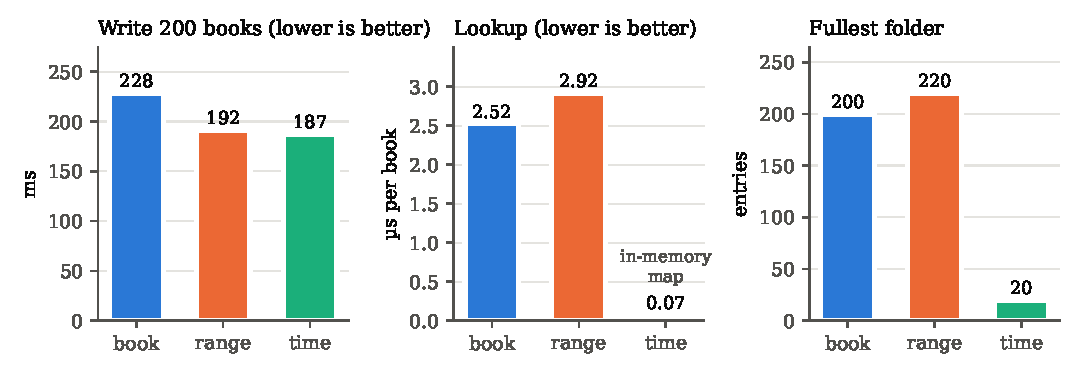
\includegraphics[width=\linewidth]{figures/datalake.pdf}
\caption{Datalake: writing, lookup and the fullest folder, 200 books.}
\end{figure}

\begin{itemize}
  \item \textbf{Writing} is dominated by the file system: the three layouts write the same 129\,MB in
        400 files, and their times differ by under 20\%.
  \item \textbf{Lookup} separates the layouts by design. \code{book} and \code{range} compute the path
        from the id and only check that both files exist. \code{time} cannot; its 0.07\us{} is an
        in-memory map of the paths this instance wrote, so it measures a hash lookup, not the layout.
  \item \textbf{Folder size} is where \code{time} wins: at most 20 entries per folder, because the
        folders follow the arrival rate rather than the ids. \code{book} has one root entry per book,
        and \code{range} already holds 220 files in its fullest folder, up to 2,000 once a range fills.
  \item \textbf{Recovery} is safe in all three: the 20 damaged books were found through
        \code{list\_book\_ids} and written again, with nothing lost or duplicated.
\end{itemize}

\subsection{Metadata benchmark}
\begin{table}[H]
\centering\small
\begin{tabular}{@{}llrrrr@{}}
\toprule
Variant & Rows & Insert (rows/s) & By id (\us) & By author (\us) & By title (\us) \\
\midrule
\code{sqlite} & 1,000 & 462,330 & 8.1 & 12.3 & 9.5 \\
 & 10,000 & 507,759 & 8.8 & 13.1 & 10.5 \\
 & 100,000 & 454,570 & 9.0 & 15.4 & 12.7 \\
\code{sqlite\_no\_index} & 1,000 & 932,219 & 7.9 & 44.3 & 41.3 \\
 & 10,000 & 1,005,172 & 8.8 & 349.8 & 327.5 \\
 & 100,000 & 915,179 & 9.3 & 5,869.3 & 5,726.1 \\
\bottomrule
\end{tabular}
\caption{Metadata: insertion in batches of 1,000 rows, and the mean time per query over 1,000 queries of each type.}
\end{table}

\begin{figure}[H]
\centering
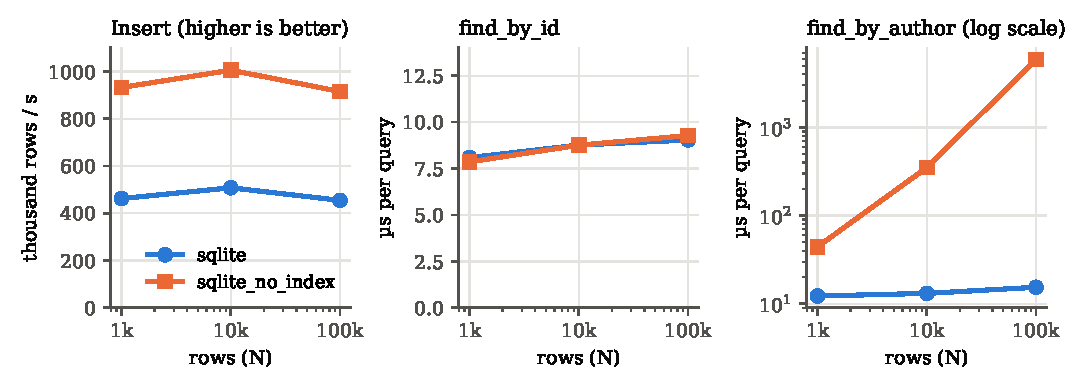
\includegraphics[width=\linewidth]{figures/metadata.pdf}
\caption{Metadata: insertion and lookups as the table grows (logarithmic row axis).}
\end{figure}

\begin{itemize}
  \item \textbf{The indexes are what keep lookups flat.} With them, a lookup by author takes 12--15\us{}
        whatever the size; without them it grows with the table, to 5.9\,ms at 100,000 rows, about 380
        times slower.
  \item \textbf{Lookups by id do not depend on them}: the primary key serves them at 8--9\us{} in both
        variants.
  \item \textbf{Their price is paid on insertion}: maintaining the two indexes halves the insertion
        rate, from about 930,000 to about 460,000 rows per second.
\end{itemize}

\subsection{Inverted-index benchmark}
\begin{table}[H]
\centering\small
\begin{tabular}{@{}lrrrrrr@{}}
\toprule
Structure & \multicolumn{3}{c}{Build (ms)} & \multicolumn{3}{c}{Query (\us)} \\
\cmidrule(lr){2-4}\cmidrule(lr){5-7}
 & $N=50$ & 100 & 200 & 50 & 100 & 200 \\
\midrule
\code{monolithic} & 282 & 709 & 1,849 & 0.85 & 0.97 & 1.42 \\
\code{hierarchical} & 2,194 & 3,482 & 6,546 & 14.5 & 16.1 & 22.0 \\
\code{mongo} & 968 & 1,683 & 3,359 & 266.6 & 235.3 & 314.6 \\
\bottomrule
\end{tabular}
\caption{Building the whole index, and the mean time of an AND query over 100 rounds of the shared workload.}
\end{table}

\begin{figure}[H]
\centering
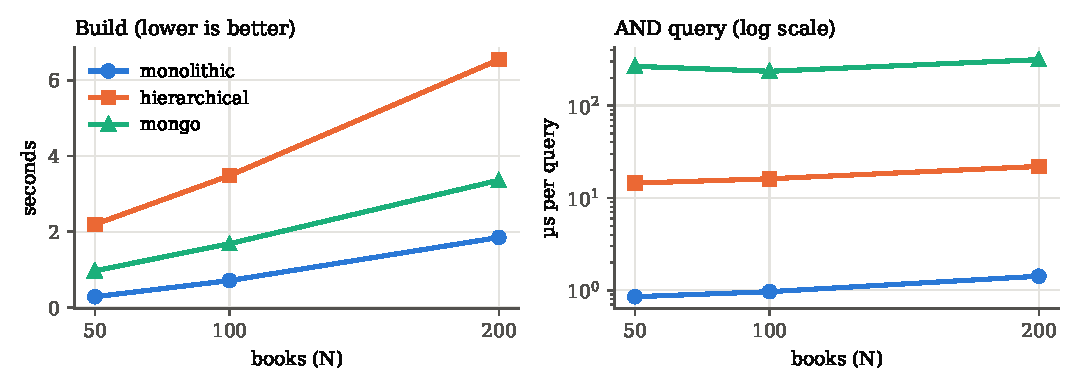
\includegraphics[width=\linewidth]{figures/index_build_query.pdf}
\caption{Index build and query time as the collection grows.}
\end{figure}

\begin{table}[H]
\centering\small
\begin{tabular}{@{}lrrrrrr@{}}
\toprule
Structure & \multicolumn{3}{c}{Add one book (ms)} & \multicolumn{3}{c}{Memory (MB)} \\
\cmidrule(lr){2-4}\cmidrule(lr){5-7}
 & $N=50$ & 100 & 200 & 50 & 100 & 200 \\
\midrule
\code{monolithic} & 93 & 165 & 300 & 16.3 & 28.1 & 54.1 \\
\code{hierarchical} & 330 & 386 & 482 & 0.0 & 0.0 & 0.0 \\
\code{mongo} & 645 & 685 & 922 & 0.01 & 0.01 & 0.01 \\
\bottomrule
\end{tabular}
\caption{Adding the last 10\% of the books one at a time to an index of the rest, and the memory in use after opening a written structure for reading (\code{heap\_after\_open}).}
\end{table}

\begin{figure}[H]
\centering
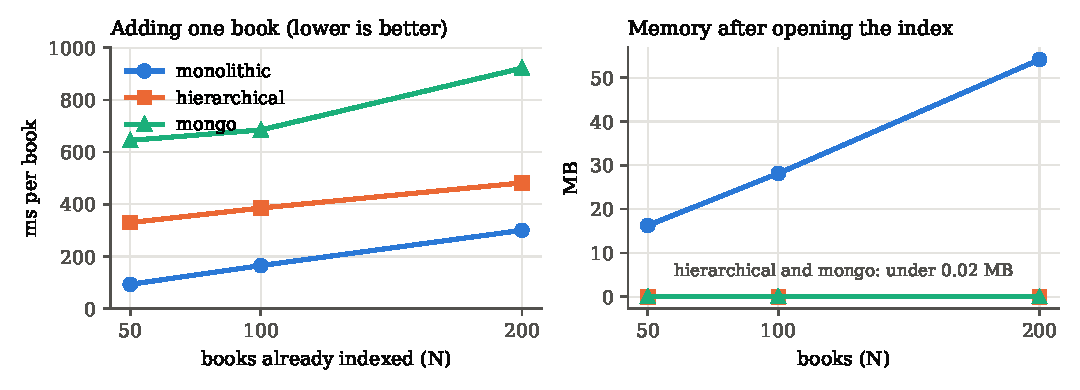
\includegraphics[width=\linewidth]{figures/index_update_memory.pdf}
\caption{Cost of adding a book, and memory held by an opened index.}
\end{figure}

\begin{table}[H]
\centering\small
\begin{tabular}{@{}lrrrr@{}}
\toprule
Structure & Bytes & Files & Allocated bytes & Allocated / bytes \\
\midrule
\code{monolithic} & 8,893,537 & 1 & 8,900,608 & 1.0 \\
\code{hierarchical} & 7,251,967 & 129,356 & 529,993,728 & 73.1 \\
\code{mongo} & 13,910,016 & --- & --- & --- \\
\bottomrule
\end{tabular}
\caption{The index on disk, $N = 200$: 129,356 terms and 1,581,064 postings in every structure. For \code{mongo}, the bytes are the collection's storage plus its indexes, as reported by MongoDB.}
\end{table}

\begin{figure}[H]
\centering
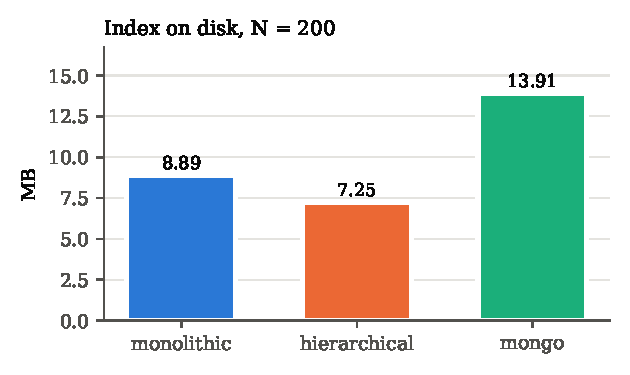
\includegraphics[width=0.6\linewidth]{figures/index_disk.pdf}
\caption{Index size on disk, $N = 200$.}
\end{figure}

\begin{itemize}
  \item \textbf{\code{monolithic} is the fastest index to build and to query}: 1.4\us{} per query at
        $N = 200$, 15 times faster than \code{hierarchical} and over 200 times faster than \code{mongo},
        whose every lookup is a round trip to the server.
  \item \textbf{But it is the only structure whose costs grow with the whole index.} Adding a book
        rewrites the entire JSON file (93 $\rightarrow$ 300\,ms as $N$ quadruples), and opening it
        loads every posting list (16 $\rightarrow$ 54\,MB). \code{hierarchical} and \code{mongo} touch
        only the new book's terms and keep almost nothing in memory.
  \item \textbf{\code{hierarchical} has the smallest data but the largest footprint.} Its 7.25\,MB of
        postings sit in 129,356 small files, and every file takes at least one 4\,KB block: 530\,MB
        reserved, 73 times the data.
  \item \textbf{Building always holds the whole index in memory}: about 92--97\,MB at $N = 200$ for any
        structure, because every writer persists one complete in-memory \code{InvertedIndex}.
\end{itemize}

\subsection{Summary: which structure to choose}
\begin{table}[H]
\centering\small
\begin{tabularx}{\linewidth}{@{}L{2.6cm} L{3.0cm} Y@{}}
\toprule
Part & Choice & Because \\
\midrule
Datalake & \code{book} & Fastest lookup that survives a restart, fastest change detection and recovery; identical bytes. Move to \code{range} for a far larger collection, to bound the folders. \\
Inverted index & \code{monolithic} & Fastest build, queries and updates at 200 books. Move to \code{hierarchical} at roughly 700 books, where its per-term updates become cheaper and the monolithic file's memory keeps growing. \\
Metadata & \code{sqlite} with both indexes & Lookups by author and title stay flat as the table grows, for half the insertion rate. \\
\bottomrule
\end{tabularx}
\caption{Structures selected for the final implementation.}
\end{table}

% ================================================================ 8
\section{Conclusions and future improvements}

\subsection{Conclusions}
\begin{itemize}
  \item The C++ module implements the whole Stage~1 data layer: downloading and splitting,
        three datalake layouts, SQLite metadata, three index structures, AND queries and a control
        layer that resumes without losing or repeating books.
  \item It follows the common contract exactly: byte-identical split books, the reference term and
        posting counts, and the SPEC result format for all 12 experiments.
  \item Interfaces, factories and dependency injection let every structure be swapped by
        configuration, and let 232 tests run without network or real data.
  \item The benchmarks justify \code{book} + \code{monolithic} at this scale and say when to change:
        \code{monolithic}'s update cost and memory grow with the index, and \code{hierarchical}'s
        per-term files waste disk blocks but keep updates and memory bounded.
  \item Running the experiments on real data found and fixed real problems: missing transaction
        batching in SQLite, a whole-index rewrite on every update, a hierarchical index that left
        stale files, per-term round trips to MongoDB, and a stale collection a plain existence check
        trusted.
\end{itemize}

\subsection{Limitations and future improvements}
\begin{itemize}
  \item \textbf{\code{time} lookups last one process.} A lookup that survives a restart would scan the
        day and hour folders, or keep a persistent id-to-path map.
  \item \textbf{Datalake writes are not atomic.} The module relies on the control layer's
        write-first, mark-after rule; writing to a temporary file and renaming it would also protect
        a single file.
  \item \textbf{Start-up cost grows with the dataset.} The in-memory index is rebuilt from every
        indexed book on each run; reading it back from the persisted structure would avoid that.
  \item \textbf{The command-line wiring has no unit tests}, and five pipeline tests share temporary
        folder names, so the suite runs sequentially.
  \item \textbf{Each MongoDB call opens a new connection}; keeping one client per writer would remove
        that cost.
  \item \textbf{Only the two structure keys are configurable}; paths, the MongoDB URI and HTTP timeouts
        are not, and downloads set no timeout.
  \item \textbf{Growth.} Past a few hundred books the index should move to \code{hierarchical}, and a
        collection the size of the Gutenberg catalogue would call for the \code{range} layout.
\end{itemize}

\end{document}
